% answers.tex —— 2009 年·普通高等学校招生考试·上海卷·文科 · 参考答案与详细解析片段
% 由 tools/generate_projects.py 依来源总账自 2009/2009_数学真题_上海文_试题.md + 2009/2009_数学真题_上海文_解析正文.md + 2009/2009_数学真题_上海文_答案要点.md 生成，勿手改（改源 MD 后重跑）


\begin{gktip}
固定候选 PDF 仅含题面，无答案、解析和评分标准，原卷亦未标注分值；以下为非官方编者独立推导，官方答案字段为空。题面文字层只作定位，公式、上下标与三幅图（Q4 程序框图、Q5 正四棱柱、Q16 三视图）均以 300/400 dpi 原页复核后重绘。
\end{gktip}

\begin{answer}
\gksolhead{1}{}

\textbf{题目}：

函数 $f(x)=x^3+1$ 的反函数 $f^{-1}(x)=$\gkblank{}．

\Needspace{4\baselineskip}
\textbf{解析}

\Needspace{5\baselineskip}
$y=x^3+1$，则 $x^3=y-1$，$x=\sqrt[3]{y-1}$。故

\nopagebreak[4]
\[f^{-1}(x)=\sqrt[3]{x-1}\quad(x\in\mathbf R).\]

\gkanswer{答案：$\sqrt[3]{x-1}$（$x\in\mathbf R$）。}

\end{answer}
\begin{answer}
\gksolhead{2}{}

\textbf{题目}：

已知集合 $A=\{x\mid x\leqslant1\}$，$B=\{x\mid x\geqslant a\}$，且 $A\cup B=\mathbf R$，则实数 $a$ 的取值范围是\gkblank{}．

\Needspace{4\baselineskip}
\textbf{解析}

$A=(-\infty,1]$，$B=[a,+\infty)$。并集覆盖全体实数，需 $a\leqslant1$。

（若 $a>1$，则区间 $(1,a)$ 中的数既不在 $A$ 也不在 $B$。）

\gkanswer{答案：$a\leqslant1$。}

\end{answer}
\begin{answer}
\gksolhead{3}{}

\textbf{题目}：

若行列式 $\begin{vmatrix}4&5&x\\1&x&3\\7&8&9\end{vmatrix}$ 中，元素 $4$ 的代数余子式大于 $0$，则 $x$ 满足的条件是\gkblank{}．

\Needspace{4\baselineskip}
\textbf{解析}

\Needspace{5\baselineskip}
元素 $4$ 在第 $1$ 行第 $1$ 列，其代数余子式为

\nopagebreak[4]
\[(-1)^{1+1}\begin{vmatrix}x&3\\8&9\end{vmatrix}=9x-24 .\]

\Needspace{5\baselineskip}
由 $9x-24>0$ 得

\nopagebreak[4]
\[x>\frac83 .\]

\gkanswer{答案：$x>\frac83$。}

\end{answer}
\begin{answer}
\gksolhead{4}{}

\textbf{题目}：

某算法的程序框图如图所示，则输出量 $y$ 与输入量 $x$ 满足的关系式是\gkblank{}．
\nopagebreak[4]
\begin{center}% 2009 年上海卷文科第 4 题：算法程序框图。
% 来源 PDF：普通高考/2009/2009上海文.pdf，SHA256 5212f16aacbac7b10c5df44f90ccd94ba0218c31c04bd0c4e9e0e8f0284ca5f3
% 原页：第 1 页（A3 三栏）第 1 栏，印刷页 555，图在题干下方。
% 重绘依据：自上而下「开始」→「输入实数 x」→ 判断菱形「x>1」；
%   是（向下）→「y←x−2」，否（向右再向下）→「y←2^x」；两路汇合 →「输出 y」→「结束」。
\begin{tikzpicture}[scale=0.95, semithick, >=Stealth,
  node distance=6mm, every node/.style={inner sep=4pt, font=\small}]
  \node (start) [draw, rounded corners=4pt, minimum width=2.2cm, minimum height=0.7cm] {开始};
  \node (input) [draw, trapezium, trapezium left angle=70, trapezium right angle=110,
    minimum width=4.0cm, minimum height=0.8cm, below=of start] {输入实数 $x$};
  \node (cond) [draw, diamond, aspect=2.2, minimum width=4.2cm, minimum height=1.2cm,
    below=of input] {$x>1$};
  \node (yes) [draw, minimum width=2.6cm, minimum height=0.8cm,
    below=of cond, xshift=-2.1cm] {$y\leftarrow x-2$};
  \node (no) [draw, minimum width=2.6cm, minimum height=0.8cm,
    below=of cond, xshift=2.6cm] {$y\leftarrow 2^{x}$};
  \node (output) [draw, trapezium, trapezium left angle=70, trapezium right angle=110,
    minimum width=3.6cm, minimum height=0.8cm, below=of yes, xshift=2.3cm] {输出 $y$};
  \node (end) [draw, rounded corners=4pt, minimum width=2.2cm, minimum height=0.7cm,
    below=of output] {结束};
  \draw[->] (start) -- (input);
  \draw[->] (input) -- (cond);
  \draw[->] (cond) -- node[left, xshift=-1pt] {是} (yes);
  \draw[->] (cond) -- node[above, yshift=1pt] {否} (no);
  \draw[->] (yes) -- (output);
  \draw[->] (no) |- (output);
  \draw[->] (output) -- (end);
\end{tikzpicture}
\end{center}
\nopagebreak[4]
\Needspace{4\baselineskip}
\textbf{解析}

\Needspace{5\baselineskip}
程序框：输入 $x$ 后判断 $x>1$。成立时执行 $y\leftarrow x-2$；不成立时执行 $y\leftarrow2^x$。故

\nopagebreak[4]
\[y=\begin{cases}x-2,&x>1,\\2^x,&x\leqslant1.\end{cases}\]

\gkanswer{答案：$y=\begin{cases}x-2,&x>1,\\2^x,&x\leqslant1.\end{cases}$}

\end{answer}
\begin{answer}
\gksolhead{5}{}

\textbf{题目}：

如图，若正四棱柱 $ABCD-A_1B_1C_1D_1$ 的底面边长为 $2$，高为 $4$，则异面直线 $BD_1$ 与 $AD$ 所成角的大小是\gkblank{}．（结果用反三角函数表示）
\nopagebreak[4]
\begin{center}% 2009 年上海卷文科第 5 题：正四棱柱 ABCD-A_1B_1C_1D_1，底面边长 2、高 4。
% 来源 PDF：普通高考/2009/2009上海文.pdf，SHA256 5212f16aacbac7b10c5df44f90ccd94ba0218c31c04bd0c4e9e0e8f0284ca5f3
% 原页：第 1 页（A3 三栏）第 1 栏下部，印刷页 555，图在题干下方。
% 重绘依据：斜投影正四棱柱，A 左下、B 右下、D 左后、C 右后；上底同名加下标 1；
%   可见棱实线，被遮棱 D-D_1、C-D、D-A 虚线；BD_1 画虚线、AD 为底面边。
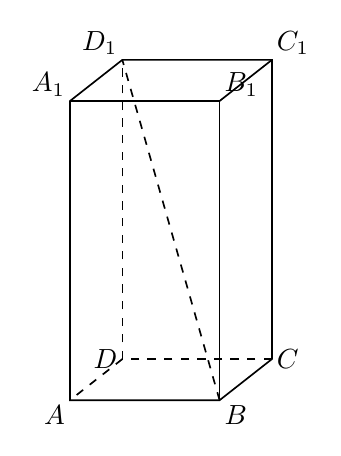
\begin{tikzpicture}[scale=0.95, semithick, every node/.style={inner sep=1.5pt}]
  \coordinate (A)  at (0,0);
  \coordinate (B)  at (2,0);
  \coordinate (D)  at (0.7,0.55);
  \coordinate (C)  at (2.7,0.55);
  \coordinate (A1) at (0,4);
  \coordinate (B1) at (2,4);
  \coordinate (D1) at (0.7,4.55);
  \coordinate (C1) at (2.7,4.55);
  \draw[dashed] (D) -- (D1);
  \draw[dashed] (C) -- (D);
  \draw[dashed] (D) -- (A);
  \draw (A) -- (B) -- (C) -- (C1) -- (D1) -- (A1) -- cycle;
  \draw (A) -- (A1);
  \draw (B) -- (B1);
  \draw (C) -- (C1);
  \draw (B1) -- (C1);
  \draw (A1) -- (B1);
  \draw[dashed] (B) -- (D1);
  \node[anchor=north east] at (A)  {$A$};
  \node[anchor=north west] at (B)  {$B$};
  \node[anchor=west]       at (C)  {$C$};
  \node[anchor=east]       at (D)  {$D$};
  \node[anchor=south east] at (A1) {$A_1$};
  \node[anchor=south west] at (B1) {$B_1$};
  \node[anchor=south west] at (C1) {$C_1$};
  \node[anchor=south east] at (D1) {$D_1$};
\end{tikzpicture}
\end{center}
\nopagebreak[4]
\Needspace{4\baselineskip}
\textbf{解析}

\Needspace{5\baselineskip}
设 $A(0,0,0)$、$B(2,0,0)$、$D(0,2,0)$、$D_1(0,2,4)$。则

\nopagebreak[4]
\[\overrightarrow{BD_1}=(-2,2,4),\qquad \overrightarrow{AD}=(0,2,0).\]

\Needspace{5\baselineskip}
两异面直线所成角为

\nopagebreak[4]
\[\cos\theta=\frac{|\overrightarrow{BD_1}\cdot\overrightarrow{AD}|}{|\overrightarrow{BD_1}||\overrightarrow{AD}|}
=\frac{4}{\sqrt{4+4+16}\cdot2}
=\frac{4}{2\sqrt6\cdot2}=\frac{1}{\sqrt6}=\frac{\sqrt6}{6}.\]

故所成角为 $\arccos\frac{\sqrt6}{6}$。

\gkanswer{答案：$\arccos\frac{\sqrt6}{6}$。}

\end{answer}
\begin{answer}
\gksolhead{6}{}

\textbf{题目}：

若球 $O_1$、$O_2$ 表面积之比 $\dfrac{S_1}{S_2}=4$，则它们的半径之比 $\dfrac{R_1}{R_2}=$\gkblank{}．

\Needspace{4\baselineskip}
\textbf{解析}

\Needspace{5\baselineskip}
球表面积 $S=4\pi R^2$，故

\nopagebreak[4]
\[\frac{S_1}{S_2}=\left(\frac{R_1}{R_2}\right)^2=4\ \Longrightarrow\ \frac{R_1}{R_2}=2 .\]

\gkanswer{答案：$2$。}

\end{answer}
\begin{answer}
\gksolhead{7}{}

\textbf{题目}：

已知实数 $x$、$y$ 满足 $\begin{cases}y\leqslant2x,\\ y\geqslant-2x,\\ x\leqslant3,\end{cases}$ 则目标函数 $z=x-2y$ 的最小值是\gkblank{}．

\Needspace{4\baselineskip}
\textbf{解析}

\Needspace{5\baselineskip}
约束为 $y\leqslant2x$、$y\geqslant-2x$、$x\leqslant3$。由 $-2x\leqslant y\leqslant2x$ 知 $x\geqslant0$，可行域为三角形，顶点为 $(0,0)$、$(3,6)$、$(3,-6)$。

\nopagebreak[4]
\[z=x-2y:\quad z(0,0)=0,\quad z(3,6)=3-12=-9,\quad z(3,-6)=3+12=15 .\]

最小值为 $-9$。

\gkanswer{答案：$-9$。}

\end{answer}
\begin{answer}
\gksolhead{8}{}

\textbf{题目}：

若等腰直角三角形的直角边长为 $2$，则以一直角边所在的直线为轴旋转一周所成的几何体体积是\gkblank{}．

\Needspace{4\baselineskip}
\textbf{解析}

\Needspace{5\baselineskip}
以直角边所在直线为轴旋转等腰直角三角形，所得为圆锥：底面半径 $r=2$，高 $h=2$。

\nopagebreak[4]
\[V=\frac13\pi r^2h=\frac13\pi\cdot4\cdot2=\frac{8\pi}{3}.\]

\gkanswer{答案：$\frac{8\pi}{3}$。}

\end{answer}
\begin{answer}
\gksolhead{9}{}

\textbf{题目}：

过点 $A(1,0)$ 作倾斜角为 $\dfrac{\pi}{4}$ 的直线，与抛物线 $y^2=2x$ 交于 $M$、$N$ 两点，则 $|MN|=$\gkblank{}．

\Needspace{4\baselineskip}
\textbf{解析}

\Needspace{5\baselineskip}
倾斜角 $\frac{\pi}{4}$，过 $A(1,0)$ 的直线为 $y=x-1$。代入 $y^2=2x$：

\nopagebreak[4]
\[(x-1)^2=2x\ \Longrightarrow\ x^2-4x+1=0 .\]

\Needspace{5\baselineskip}
设交点横坐标 $x_1,x_2$，则 $x_1+x_2=4$、$x_1x_2=1$，

\nopagebreak[4]
\[|x_1-x_2|=\sqrt{(x_1+x_2)^2-4x_1x_2}=\sqrt{16-4}=2\sqrt3 .\]

\Needspace{5\baselineskip}
直线斜率为 $1$，故

\nopagebreak[4]
\[|MN|=\sqrt{1^2+1^2}\,|x_1-x_2|=\sqrt2\cdot2\sqrt3=2\sqrt6 .\]

\gkanswer{答案：$2\sqrt6$。}

\end{answer}
\begin{answer}
\gksolhead{10}{}

\textbf{题目}：

函数 $y=2\cos^2x+\sin2x$ 的最小值是\gkblank{}．

\Needspace{4\baselineskip}
\textbf{解析}

\nopagebreak[4]
\[y=2\cos^2x+\sin2x=1+\cos2x+\sin2x
=1+\sqrt2\sin\left(2x+\frac\pi4\right).\]

\Needspace{5\baselineskip}
故最小值为

\nopagebreak[4]
\[1-\sqrt2 .\]

\gkanswer{答案：$1-\sqrt2$。}

\end{answer}
\begin{answer}
\gksolhead{11}{}

\textbf{题目}：

若某学校要从 $5$ 名男生和 $2$ 名女生中选出 $3$ 人作为上海世博会的志愿者，则选出的志愿者中男女生均不少于 $1$ 名的概率是\gkblank{}．（结果用最简分数表示）

\Needspace{4\baselineskip}
\textbf{解析}

从 $7$ 人中选 $3$ 人，共 $\mathrm C_7^3=35$ 种。

\Needspace{5\baselineskip}
全为男生：$\mathrm C_5^3=10$ 种；全为女生不可能（只有 $2$ 名女生）。故男女生均不少于 $1$ 名的选法为

\nopagebreak[4]
\[35-10=25,\]

\Needspace{5\baselineskip}
概率

\nopagebreak[4]
\[P=\frac{25}{35}=\frac57 .\]

\gkanswer{答案：$\frac57$。}

\end{answer}
\begin{answer}
\gksolhead{12}{}

\textbf{题目}：

已知 $F_1$、$F_2$ 是椭圆 $C:\dfrac{x^2}{a^2}+\dfrac{y^2}{b^2}=1$（$a>b>0$）的两个焦点，$P$ 为椭圆 $C$ 上一点，且 $\overrightarrow{PF_1}\perp\overrightarrow{PF_2}$．若 $\triangle PF_1F_2$ 的面积为 $9$，则 $b=$\gkblank{}．

\Needspace{4\baselineskip}
\textbf{解析}

\Needspace{5\baselineskip}
设 $|PF_1|=m$、$|PF_2|=n$。由 $PF_1\perp PF_2$，

\nopagebreak[4]
\[m^2+n^2=|F_1F_2|^2=(2c)^2=4c^2 .\]

\Needspace{5\baselineskip}
又椭圆定义给出 $m+n=2a$，故

\nopagebreak[4]
\[4a^2=(m+n)^2=m^2+n^2+2mn=4c^2+2mn
\ \Longrightarrow\ mn=2(a^2-c^2)=2b^2 .\]

\Needspace{5\baselineskip}
面积

\nopagebreak[4]
\[S=\frac12mn=b^2=9\ \Longrightarrow\ b=3 .\]

\gkanswer{答案：$3$。}

\end{answer}
\begin{answer}
\gksolhead{13}{}

\textbf{题目}：

已知函数 $f(x)=\sin x+\tan x$．项数为 $27$ 的等差数列 $\{a_n\}$ 满足 $a_n\in\left(-\dfrac{\pi}{2},\dfrac{\pi}{2}\right)$，且公差 $d\neq0$．若 $f(a_1)+f(a_2)+\cdots+f(a_{27})=0$，则当 $k=$\gkblank{}时，$f(a_k)=0$．

\Needspace{4\baselineskip}
\textbf{解析}

$f(x)=\sin x+\tan x$ 在 $\left(-\frac\pi2,\frac\pi2\right)$ 上为奇函数且严格递增。

27 项等差数列的中项为 $a_{14}$，且 $a_i+a_{28-i}=2a_{14}$。

若 $a_{14}=0$，则 $a_{28-i}=-a_i$，由 $f$ 为奇函数得 $f(a_i)+f(a_{28-i})=0$，故总和为 $0$。

\Needspace{5\baselineskip}
反之，若总和为 $0$，由于 $f$ 严格递增且为奇函数，各项必须成对互为相反数，故中项 $a_{14}=0$。因此

\nopagebreak[4]
\[k=14 .\]

\gkanswer{答案：$14$。}

\end{answer}
\begin{answer}
\gksolhead{14}{}

\textbf{题目}：

某地街道呈现东—西、南—北向的网格状，相邻街距都为 $1$，两街道相交的点称为格点．若以互相垂直的两条街道为轴建立直角坐标系，现有下述格点 $(-2,2)$，$(3,1)$，$(3,4)$，$(-2,3)$，$(4,5)$ 为报刊零售点．请确定一个格点\gkblank{}为发行站，使 $5$ 个零售点沿街道到发行站之间路程的和最短．

\Needspace{4\baselineskip}
\textbf{解析}

沿街道路程为曼哈顿距离，$x$、$y$ 两个方向可分离，分别取中位数。

横坐标：$-2,3,3,-2,4$，排序后为 $-2,-2,3,3,4$，中位数 $3$。

纵坐标：$2,1,4,3,5$，排序后为 $1,2,3,4,5$，中位数 $3$。

\Needspace{5\baselineskip}
故发行站取

\nopagebreak[4]
\[(3,3).\]

（核对总路程：$6+2+1+5+3=17$。）

\gkanswer{答案：$(3,3)$。}

\end{answer}
\begin{answer}
\gksolhead{15}{}

\textbf{题目}：

已知直线 $l_1:(k-3)x+(4-k)y+1=0$ 与 $l_2:2(k-3)x-2y+3=0$ 平行，则 $k$ 的值是（　）

（A）$1$ 或 $3$

（B）$1$ 或 $5$

（C）$3$ 或 $5$

（D）$1$ 或 $2$

\Needspace{4\baselineskip}
\textbf{解析}

\Needspace{5\baselineskip}
两直线平行需 $A_1B_2-A_2B_1=0$：

\nopagebreak[4]
\[(k-3)\cdot(-2)-2(k-3)(4-k)=0
\ \Longrightarrow\ (k-3)\left[-2-2(4-k)\right]=0
\ \Longrightarrow\ (k-3)(2k-10)=0 .\]

故 $k=3$ 或 $k=5$，选 C。

（$k=3$ 时两直线分别为 $y+1=0$ 与 $-2y+3=0$，均水平；$k=5$ 时分别为 $2x-y+1=0$ 与 $4x-2y+3=0$，斜率均为 $2$。）

\gkanswer{答案：C。}

\end{answer}
\begin{answer}
\gksolhead{16}{}

\textbf{题目}：

如图，已知三棱锥的底面是直角三角形，直角边长分别为 $3$ 和 $4$，过直角顶点的侧棱长为 $4$，且垂直于底面，该三棱锥的主视图是（　）
\nopagebreak[4]
\begin{center}% 2009 年上海卷文科第 16 题：底面为直角三角形、侧棱垂直于底面的三棱锥及其主视图四选项。
% 来源 PDF：普通高考/2009/2009上海文.pdf，SHA256 5212f16aacbac7b10c5df44f90ccd94ba0218c31c04bd0c4e9e0e8f0284ca5f3
% 原页：第 1 页（A3 三栏）第 2 栏下部，印刷页 555。
% 重绘依据：上方小图为三棱锥与坐标轴（z 向上、x 向前左、y 向右），底面直角边 3、4，
%   直角顶点处侧棱高 4；下方四选项为直角三角形轮廓：(A) 4×4、(B) 3×4、(C) 3×4
%   （直角在右上）、(D) 斜边 5、高 4；标注与直角记号按原图。
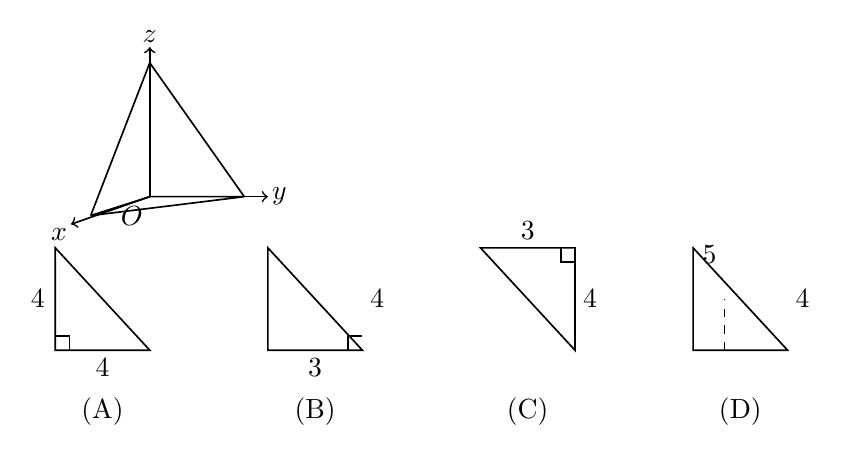
\begin{tikzpicture}[scale=1.0, semithick, every node/.style={inner sep=1.2pt}]
  % ---------- 上方立体示意 ----------
  \coordinate (O) at (1.2,0.5);
  \draw[->] (O) -- (0.2,0.15) node[anchor=north east] {$x$};
  \draw[->] (O) -- (2.7,0.5) node[anchor=west] {$y$};
  \draw[->] (O) -- (1.2,2.4) node[anchor=south] {$z$};
  \coordinate (P) at (1.2,2.2);
  \coordinate (X) at (0.45,0.26);
  \coordinate (Y) at (2.4,0.5);
  \draw (O) -- (X) -- (Y) -- cycle;
  \draw (P) -- (X);
  \draw (P) -- (Y);
  \draw (P) -- (O);
  \node[anchor=north east] at ([xshift=-1pt,yshift=-2pt]O) {$O$};
  % ---------- 四个选项 ----------
  \foreach \dx/\opt in {0/A, 2.7/B, 5.4/C, 8.1/D} {
    \node[anchor=north] at (\dx+0.6,-2.0) {(\opt)};
  }
  % (A) 4 x 4，直角在左下
  \draw (0,-0.15) -- (0,-1.45) -- (1.2,-1.45) -- cycle;
  \draw (0.18,-1.45) -- (0.18,-1.27) -- (0,-1.27);
  \node[anchor=east] at (-0.08,-0.8) {$4$};
  \node[anchor=north] at (0.6,-1.5) {$4$};
  % (B) 3 x 4，直角在右下
  \draw (2.7,-0.15) -- (2.7,-1.45) -- (3.9,-1.45) -- cycle;
  \draw (3.72,-1.45) -- (3.72,-1.27) -- (3.9,-1.27);
  \node[anchor=west] at (3.95,-0.8) {$4$};
  \node[anchor=north] at (3.3,-1.5) {$3$};
  % (C) 上边 3、右边 4，直角在右上
  \draw (5.4,-0.15) -- (6.6,-0.15) -- (6.6,-1.45) -- cycle;
  \draw (6.42,-0.15) -- (6.42,-0.33) -- (6.6,-0.33);
  \node[anchor=south] at (6.0,-0.1) {$3$};
  \node[anchor=west] at (6.65,-0.8) {$4$};
  % (D) 斜边 5、高 4，直角在右下
  \draw (8.1,-0.15) -- (8.1,-1.45) -- (9.3,-1.45) -- cycle;
  \draw[dashed] (8.5,-1.45) -- (8.5,-0.8);
  \node[anchor=south east] at (8.45,-0.4) {$5$};
  \node[anchor=west] at (9.35,-0.8) {$4$};
\end{tikzpicture}
\end{center}
\nopagebreak[4]
\Needspace{4\baselineskip}
\textbf{解析}

主视图从正面观察，看到的是底面直角边 $3$ 所对应的宽度与侧棱 $4$ 所对应的高。故主视图为直角边 $3$、$4$ 的直角三角形，选 B。

（底面的另一条直角边 $4$ 在主视方向被压缩为深度，不反映为宽度。视角约定说明：若沿另一条直角边投影，会得到 $4\times4$ 的三角形（选项 A）；本库按公开官方答案取 B。）

\gkanswer{答案：B。}

\end{answer}
\begin{answer}
\gksolhead{17}{}

\textbf{题目}：

点 $P(4,-2)$ 与圆 $x^2+y^2=4$ 上任一点连线的中点轨迹方程是（　）

（A）$(x-2)^2+(y+1)^2=1$

（B）$(x-2)^2+(y+1)^2=4$

（C）$(x+4)^2+(y-2)^2=4$

（D）$(x+2)^2+(y-1)^2=1$

\Needspace{4\baselineskip}
\textbf{解析}

\Needspace{5\baselineskip}
设圆上点 $Q(x_0,y_0)$，$P(4,-2)$，中点 $M(x,y)$：

\nopagebreak[4]
\[x=\frac{x_0+4}{2},\quad y=\frac{y_0-2}{2}
\ \Longrightarrow\ x_0=2x-4,\quad y_0=2y+2 .\]

\Needspace{5\baselineskip}
代入圆方程 $x_0^2+y_0^2=4$：

\nopagebreak[4]
\[(2x-4)^2+(2y+2)^2=4
\ \Longrightarrow\ (x-2)^2+(y+1)^2=1 .\]

选 A。

\gkanswer{答案：A。}

\end{answer}
\begin{answer}
\gksolhead{18}{}

\textbf{题目}：

在发生某公共卫生事件期间，有专业机构认为该事件在一段时间没有发生在规模群体感染的标志为「连续 $10$ 天，每天新增疑似病例不超过 $7$ 人」．根据过去 $10$ 天甲、乙、丙、丁四地新增疑似病例数据，一定符合该标志的是（　）

（A）甲地：总体均值为 $3$，中位数为 $4$

（B）乙地：总体均值为 $1$，总体方差大于 $0$

（C）丙地：中位数为 $2$，众数为 $3$

（D）丁地：总体均值为 $2$，总体方差为 $3$

\Needspace{4\baselineskip}
\textbf{解析}

标志要求连续 $10$ 天每天新增疑似病例不超过 $7$ 人，即不能出现 $\geqslant8$ 的数据。

丁地总体均值为 $2$、总体方差为 $3$：若某天为 $8$，该天偏差平方为 $(8-2)^2=36$，而 $10$ 天偏差平方总和仅为 $10\times3=30$，矛盾。故丁地不可能出现 $8$ 人及以上，必符合标志。

其余三项均可构造含 $8$ 的数据而不违反所述统计量（例如甲地取 $0,0,\cdots,4,8$ 可使均值 $3$、中位数 $4$），不能保证。

选 D。

\gkanswer{答案：D。}

\end{answer}
\begin{answer}
\gksolhead{19}{}

\textbf{题目}：

已知复数 $z=a+b\mathrm i$（$a,b\in\mathbf R^+$）（$\mathrm i$ 是虚数单位）是方程 $x^2-4x+5=0$ 的根．复数 $w=u+3\mathrm i$（$u\in\mathbf R$）满足 $|w-z|<2\sqrt5$，求 $u$ 的取值范围．

\Needspace{4\baselineskip}
\textbf{解析}

\Needspace{5\baselineskip}
方程 $x^2-4x+5=0$ 的根为

\nopagebreak[4]
\[x=\frac{4\pm\sqrt{16-20}}{2}=2\pm\mathrm i .\]

由 $a,b\in\mathbf R^+$，取 $z=2+\mathrm i$。

\Needspace{5\baselineskip}
$w-z=(u-2)+2\mathrm i$，故

\nopagebreak[4]
\[|w-z|^2=(u-2)^2+4<20
\ \Longrightarrow\ (u-2)^2<16
\ \Longrightarrow\ -2<u<6 .\]

\gkanswer{答案：$u\in(-2,6)$。}

\end{answer}
\begin{answer}
\gksolhead{20}{}

\textbf{题目}：

已知 $\triangle ABC$ 的角 $A$、$B$、$C$ 所对的边分别是 $a$、$b$、$c$，设向量 $\boldsymbol m=(a,b)$，$\boldsymbol n=(\sin B,\sin A)$，$\boldsymbol p=(b-2,a-2)$．

（1）若 $\boldsymbol m\parallel\boldsymbol n$，求证：$\triangle ABC$ 为等腰三角形；

（2）若 $\boldsymbol m\perp\boldsymbol p$，边长 $c=2$，角 $C=\dfrac{\pi}{3}$，求 $\triangle ABC$ 的面积．

\Needspace{4\baselineskip}
\textbf{解析}

\Needspace{5\baselineskip}
（1）$\boldsymbol m\parallel\boldsymbol n$，故

\nopagebreak[4]
\[a\sin A-b\sin B=0 .\]

\Needspace{5\baselineskip}
由正弦定理 $a=2R\sin A$、$b=2R\sin B$，得

\nopagebreak[4]
\[2R\sin^2A-2R\sin^2B=0\ \Longrightarrow\ \sin A=\sin B .\]

$A,B$ 为三角形内角，故 $A=B$ 或 $A+B=\pi$（后者不可能），所以 $A=B$，$\triangle ABC$ 为等腰三角形。

\Needspace{5\baselineskip}
（2）$\boldsymbol m\perp\boldsymbol p$，故

\nopagebreak[4]
\[a(b-2)+b(a-2)=0\ \Longrightarrow\ 2ab-2a-2b=0\ \Longrightarrow\ ab=a+b .\]

\Needspace{5\baselineskip}
由余弦定理，$c=2$、$C=\frac\pi3$：

\nopagebreak[4]
\[4=a^2+b^2-2ab\cos\frac\pi3=a^2+b^2-ab=(a+b)^2-3ab .\]

\Needspace{5\baselineskip}
令 $s=a+b=ab$，则

\nopagebreak[4]
\[s^2-3s-4=0\ \Longrightarrow\ s=4\ \text{\text{或}}\ s=-1 .\]

\Needspace{5\baselineskip}
$s>0$，故 $s=4$，$ab=4$。面积

\nopagebreak[4]
\[S=\frac12ab\sin C=\frac12\cdot4\cdot\frac{\sqrt3}{2}=\sqrt3 .\]

\gkanswer{答案：（1）证明见解析；（2）$\sqrt3$。}

\end{answer}
\begin{answer}
\gksolhead{21}{}

\textbf{题目}：

\Needspace{5\baselineskip}
有时可用函数

\nopagebreak[4]
\[f(x)=\begin{cases}0.1+15\ln\dfrac{a}{a-x},&x\leqslant6,\\[6pt] \dfrac{x-4.4}{x-4},&x>6,\end{cases}\]

描述学习某学科知识的掌握程度，其中 $x$ 表示某学科知识的学习次数（$x\in\mathbf N^*$），$f(x)$ 表示对该学科知识的掌握程度，正实数 $a$ 与学科知识有关．

（1）证明：当 $x\geqslant7$ 时，掌握程度的增加量 $f(x+1)-f(x)$ 总是下降；

（2）根据经验，学科甲、乙、丙对应的 $a$ 的取值区间分别为 $(115,121]$、$(121,127]$、$(121,133]$．当学习某学科知识 $6$ 次时，掌握程度是 $85\%$，请确定相应的学科．

\Needspace{4\baselineskip}
\textbf{解析}

\Needspace{5\baselineskip}
（1）$x\geqslant7$ 时用第二段：

\nopagebreak[4]
\[f(x)=\frac{x-4.4}{x-4}=1-\frac{0.4}{x-4}.\]

\Needspace{5\baselineskip}
于是

\nopagebreak[4]
\[f(x+1)-f(x)
=\left(1-\frac{0.4}{x-3}\right)-\left(1-\frac{0.4}{x-4}\right)
=0.4\left(\frac{1}{x-4}-\frac{1}{x-3}\right)
=-\frac{0.4}{(x-3)(x-4)} .\]

其绝对值 $\frac{0.4}{(x-3)(x-4)}$ 随 $x$ 增大而减小，且恒为负，故 $f(x+1)-f(x)$ 总是下降（趋近于 $0$）。

\Needspace{5\baselineskip}
（2）$x=6$ 时用第一段：

\nopagebreak[4]
\[0.1+15\ln\frac{a}{a-6}=0.85
\ \Longrightarrow\ \ln\frac{a}{a-6}=0.05 .\]

\Needspace{5\baselineskip}
故

\nopagebreak[4]
\[\frac{a}{a-6}=\mathrm e^{0.05}
\ \Longrightarrow\ a=\frac{6\mathrm e^{0.05}}{\mathrm e^{0.05}-1}.\]

\Needspace{5\baselineskip}
计算：$\mathrm e^{0.05}\approx1.051271$，

\nopagebreak[4]
\[a\approx\frac{6\times1.051271}{0.051271}\approx123.0 .\]

$123.0\in(121,127]$，故对应学科乙。

\begin{gktip}
源疑点：原页把丙的区间印作 $(121,133]$，与乙的 $(121,127]$ 重叠，$123.0$ 同时落在两区间内；按三区间应互斥的通常意图（丙应为 $(127,133]$），判定为乙。题面照录原页区间，登记 ISSUE，不擅自改数。
\end{gktip}

\gkanswer{答案：（1）证明见解析；（2）学科乙。}

\end{answer}
\begin{answer}
\gksolhead{22}{}

\textbf{题目}：

已知双曲线 $C$ 的中心是原点，右焦点为 $F(\sqrt3,0)$，一条渐近线 $m:x+\sqrt2y=0$．设过点 $A(-3\sqrt2,0)$ 的直线 $l$ 的方向向量 $\boldsymbol e=(1,k)$．

（1）求双曲线 $C$ 的方程；

（2）若过原点的直线 $a\parallel l$，且 $a$ 与 $l$ 的距离为 $\sqrt6$，求 $k$ 的值；

（3）证明：当 $k>\dfrac{\sqrt2}{2}$ 时，在双曲线 $C$ 的右支上不存在点 $Q$，使之到直线 $l$ 的距离为 $\sqrt6$．

\Needspace{4\baselineskip}
\textbf{解析}

\Needspace{5\baselineskip}
（1）设双曲线为 $\frac{x^2}{a^2}-\frac{y^2}{b^2}=1$。渐近线 $x+\sqrt2y=0$ 即 $y=-\frac{x}{\sqrt2}$，故

\nopagebreak[4]
\[\frac ba=\frac1{\sqrt2}\ \Longrightarrow\ b^2=\frac{a^2}{2}.\]

\Needspace{5\baselineskip}
又右焦点 $F(\sqrt3,0)$，故 $c=\sqrt3$，$a^2+b^2=3$。于是

\nopagebreak[4]
\[\frac32a^2=3\ \Longrightarrow\ a^2=2,\quad b^2=1 .\]

\Needspace{5\baselineskip}
双曲线为

\nopagebreak[4]
\[\frac{x^2}{2}-y^2=1 .\]

\Needspace{5\baselineskip}
（2）$l$ 过 $A(-3\sqrt2,0)$、方向向量 $(1,k)$，方程为

\nopagebreak[4]
\[y=k(x+3\sqrt2)\ \Longrightarrow\ kx-y+3\sqrt2k=0 .\]

\Needspace{5\baselineskip}
过原点的平行线 $a$ 为 $kx-y=0$。两平行线距离

\nopagebreak[4]
\[d=\frac{|3\sqrt2k|}{\sqrt{k^2+1}}=\sqrt6 .\]

\Needspace{5\baselineskip}
平方：

\nopagebreak[4]
\[18k^2=6(k^2+1)\ \Longrightarrow\ 12k^2=6\ \Longrightarrow\ k^2=\frac12 .\]

\Needspace{5\baselineskip}
故

\nopagebreak[4]
\[k=\pm\frac{\sqrt2}{2} .\]

\Needspace{5\baselineskip}
（3）设 $Q(x,y)$ 在右支上，则 $x\geqslant\sqrt2$，且

\nopagebreak[4]
\[y^2=\frac{x^2}{2}-1<\frac{x^2}{2}\ \Longrightarrow\ |y|<\frac{x}{\sqrt2}.\]

\Needspace{5\baselineskip}
当 $k>\frac{\sqrt2}{2}$ 时，

\nopagebreak[4]
\[kx-y\geqslant kx-|y|>\left(k-\frac1{\sqrt2}\right)x\geqslant0 .\]

\Needspace{5\baselineskip}
故 $Q$ 到 $l$ 的距离

\nopagebreak[4]
\[d(Q,l)=\frac{|kx-y+3\sqrt2k|}{\sqrt{k^2+1}}
\geqslant\frac{3\sqrt2k}{\sqrt{k^2+1}}
=\frac{3\sqrt2}{\sqrt{1+\frac1{k^2}}} .\]

\Needspace{5\baselineskip}
由 $k>\frac{\sqrt2}{2}$ 得 $k^2>\frac12$，$\frac1{k^2}<2$，故

\nopagebreak[4]
\[\sqrt{1+\frac1{k^2}}<\sqrt3
\ \Longrightarrow\ d(Q,l)>\frac{3\sqrt2}{\sqrt3}=\sqrt6 .\]

所以右支上不存在点 $Q$ 到 $l$ 的距离恰为 $\sqrt6$。

\gkanswer{答案：（1）$\frac{x^2}{2}-y^2=1$；（2）$k=\pm\frac{\sqrt2}{2}$；（3）证明见解析。}

\end{answer}
\begin{answer}
\gksolhead{23}{}

\textbf{题目}：

已知 $\{a_n\}$ 是公差为 $d$ 的等差数列，$\{b_n\}$ 是公比为 $q$ 的等比数列．

（1）若 $a_n=3n+1$，是否存在 $m$、$k\in\mathbf N^*$，有 $a_m+a_{m+1}=a_k$？请说明理由；

（2）若 $b_n=aq^n$（$a$、$q$ 为常数，且 $aq\neq0$），对任意 $m$ 存在 $k$，有 $b_m\cdot b_{m+1}=b_k$，试求 $a$、$q$ 满足的充要条件；

（3）若 $a_n=2n+1$，$b_n=3^n$，试确定所有的 $p$，使数列 $\{b_n\}$ 中存在某个连续 $p$ 项的和是数列 $\{a_n\}$ 中的一项，请证明．

\Needspace{4\baselineskip}
\textbf{解析}

\Needspace{5\baselineskip}
（1）$a_n=3n+1$，故

\nopagebreak[4]
\[a_m+a_{m+1}=(3m+1)+(3m+4)=6m+5 .\]

\Needspace{5\baselineskip}
若等于 $a_k=3k+1$，则

\nopagebreak[4]
\[3k=6m+4\ \Longrightarrow\ k=2m+\frac43\notin\mathbf N^*,\]

故不存在这样的 $m,k$。

\Needspace{5\baselineskip}
（2）$b_mb_{m+1}=a^2q^{2m+1}$，$b_k=aq^k$。条件等价于：对任意 $m\in\mathbf N^*$，存在正整数 $k$，使

\nopagebreak[4]
\[aq^{2m+1-k}=1 .\]

若 $q=1$，则 $a^2=a$，又 $a\neq0$，故 $a=1$。此时 $(a,q)=(1,1)$ 满足条件。

\Needspace{5\baselineskip}
若 $q\neq1$，则

\nopagebreak[4]
\[k=2m+1+\log_q a .\]

\Needspace{5\baselineskip}
要使每个 $m$ 对应的 $k$ 都是正整数，$\log_q a$ 必须为整数 $c$；且 $m=1$ 时 $k=3+c\geqslant1$，即 $c\geqslant-2$。此时

\nopagebreak[4]
\[a=q^c,\qquad k=2m+1+c .\]

故充要条件为：$(a,q)=(1,1)$，或 $q\neq1$ 且 $a=q^c$（$c\in\mathbf Z$，$c\geqslant-2$）。

\Needspace{5\baselineskip}
（3）设连续 $p$ 项从 $b_{m+1}$ 开始，和为

\nopagebreak[4]
\[S=3^{m+1}+3^{m+2}+\cdots+3^{m+p}
=3^{m+1}\cdot\frac{3^p-1}{2}.\]

$\{a_n\}$ 的每一项 $a_k=2k+1$ 都是奇数。

\begin{itemize}
\item 若 $p$ 为偶数，则 $3^p\equiv1\pmod4$，$3^p-1\equiv0\pmod4$，故 $\frac{3^p-1}{2}$ 为偶数，$S$ 为偶数，不可能等于 $a_k$。
\item 若 $p$ 为奇数，则 $3^p\equiv3\pmod4$，$3^p-1\equiv2\pmod4$，故 $\frac{3^p-1}{2}$ 为奇数，$S=3^{m+1}\cdot\frac{3^p-1}{2}$ 为奇数。取
\end{itemize}

\nopagebreak[4]
\[k=\frac{S-1}{2},\]

\Needspace{5\baselineskip}
则 $k$ 为正整数，且

\nopagebreak[4]
\[a_k=2k+1=S .\]

故所有正奇数 $p$ 都满足要求，偶数 $p$ 都不满足。

\gkanswer{答案：（1）不存在；（2）$(a,q)=(1,1)$，或 $q\neq1$ 且 $a=q^c$（$c\in\mathbf Z$，$c\geqslant-2$）；（3）所有正奇数 $p$。}

\end{answer}